\documentclass{article}

\usepackage{graphicx}
\usepackage{xcolor}
\usepackage{amsmath}

\title{Quantum computing TP\\ Phase estimation for chemistry}


\author{\textbf{Supervisor:} Bertrand Marchand}


\begin{document}
\maketitle
\begin{abstract}
You need to fill up the helper file and some notebook cells according to the questions.
Send the notebooks and helper files in a zip by *** 2021. They will be corrected and graded
\end{abstract}

\section{Quantum Programming Basics}

\paragraph{Question 1} Implement the following circuit, simulate it for $\theta=0.3$, and print all states along with their amplitudes and probabilities.

\begin{center}
\includegraphics[width=.7\textwidth]{qat2pdf_llce_fji_circ.pdf}
\end{center}

Where $ham\_X(\theta) = e^{-i\theta X}$ with $X=\begin{pmatrix}0 & 1 \\ 1 & 0\end{pmatrix}$

\paragraph{Hint} Define $ham\_X$ as an ``AbstractGate'', then apply it using ``.ctrl()'' to get a controlled version, as suggested in 
the ``minimal notebook''.

\section{Iterative quantum phase estimation, reproducing results from \textcolor{blue}{\cite{o2016scalable}}}

\subsection{Hamiltonian simulation}

The Hamiltonians whose ground state energy we are trying to compute are of the form: 
$$H(R) = g_{0}I+g_{1}ZI+g_{2}IZ+g_{3}ZZ+g_{4}YY+g_{5}XX $$

Because we use \textbf{Trotterization}, we will only have
to implement the unitary evolutions generated by each of the
individual terms: $e^{-iXXdt}$, $e^{-iZIdt}$, 
$e^{-iIZdt}$, $e^{-iZZdt}$, $e^{-iYYdt}$ and $e^{-iXXdt}$.

\paragraph{}
We could implement them using Abstract gates and a numerical
computation of the matrix exponential. But the computation of the
matrix exponential does not scale well with the number of qubits, 
and thus this method cannot be used in the ``general case'', when
working with a large molecule.

What we will do therefore instead is find small parametrized circuits 
implementing each of the unitary evolutions. The small circuits
may only use ``usual gates'', such as CNOTs and single-qubit Pauli
rotations, that are already pre-implemented in PyAQASM/myqlm.
We will then use \textbf{QRoutines} to paste these circuits into
the final algorithm. Such a method does yield circuits of polynomial
size for arbitrary Pauli products over $n$ qubits.

\paragraph{}
\textbf{Example}:
You can check that: $Z\otimes Z = CNOT_{0\rightarrow 1} \cdot I\otimes Z \cdot CNOT_{0\rightarrow 1} $\\~\\
with $CNOT_{0\rightarrow 1}=\begin{pmatrix} 1 & 0 & 0 & 0 \\ 0 & 1 & 0 & 0 \\ 0 & 0 & 0 & 1 \\ 0 & 0 & 1 & 0 \end{pmatrix}$, $\otimes$
the Kronecker product and $\cdot$ the standard matrix product.\\~\\
It allows us to write: 
\begin{align*}
e^{-iZZdt} &= e^{-i(CNOT_{0\rightarrow 1})\cdot (IZ)\cdot (CNOT_{0\rightarrow 1})dt}\\ 
           &= CNOT_{0\rightarrow 1}\cdot e^{-iIZdt} CNOT_{0\rightarrow 1}\\
           &= CNOT_{0\rightarrow 1}\cdot \left(I\otimes e^{-iZdt}\right)\cdot CNOT_{0\rightarrow 1}
\end{align*}
i.e:
\begin{center}
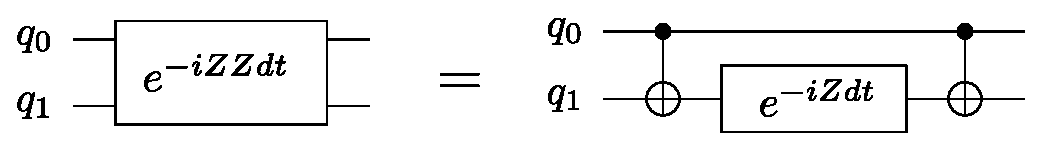
\includegraphics[width=.5\textwidth]{zz_rz.eps}
\end{center}


where $e^{-iZdt} = \begin{pmatrix} e^{-idt} & 0 \\ 0 & e^{idt} \end{pmatrix} = RZ(-dt)$.

\paragraph{} $RZ$ is a ``standard gate'', pre-implemented in PyAQASM.
Likewise, $RX$ and $RY$ are pre-implemented.

\paragraph{Question 2} Following the example above, which is already implemented in the notebook, and knowing in addition that:
$$ X\otimes X = CNOT_{0\rightarrow 1} \cdot X\otimes I \cdot 
CNOT_{0\rightarrow 1}  $$
$$ SXS^{\dagger} = Y $$ and 
$$ Y\otimes X = CNOT_{0\rightarrow 1} \cdot Y\otimes I \cdot 
CNOT_{0\rightarrow 1} $$
write down the QRoutines carrying out each of the required 
Hamiltonian simulations, by filling the templates already written
in the notebook.

\subsection{Iterative Phase estimation}

\subsubsection{Trotterization}

\textbf{Question 3} Write a function taking as input hamiltonian
coefficients, an interval of time $dt$,  and a Trotter number $p$, 
and returning a Qroutine which implements the corresponding
Trotterized implementation of the Hamiltonian.

Below where your implementation should go, a cell contains
a piece of code that tests whether the Trotterization produces
a ``reasonable'' implementation of the Hamiltonian.

\subsection{final plots}
\bibliography{biblio}
\bibliographystyle{unsrt}
\end{document}
